\documentclass[UTF8]{ctexart}
\usepackage[a4paper,margin=1.8cm]{geometry}
\usepackage{graphicx}
\usepackage{float}
\usepackage{longtable}
\usepackage{array}
\usepackage{xcolor}
\usepackage{fancyvrb}
\usepackage{hyperref}
\setlength{\parindent}{0pt}
\setlength{\parskip}{0.45em}
\begin{document}
\section*{机器无关优化完整模拟卷 06（题目与完整解析）}

\subsection*{卷面说明}

\begin{Verbatim}[fontsize=\small,breaklines=true]
考试时间：120 分钟
总分：100 分
说明：本卷独立覆盖局部优化、到达定值、活跃变量、可用表达式、复制传播、支配与自然循环。
所有 CFG、gen/kill、use/def 和表达式全集均在题面中给出。
\end{Verbatim}

\subsection*{A 卷题目}

\subsubsection*{一、语义不变优化与数据流框架（20 分）}

给定基本块：

\begin{Verbatim}[fontsize=\small,breaklines=true]
(1) t1 = a + b
(2) t2 = a + b
(3) x  = t2
(4) y  = x
(5) z  = 3 * 4
\end{Verbatim}

块出口只有 \texttt{x} 活跃。

1. 指出公共子表达式并消除。 2. 对复制语句做传播。 3. 对常量表达式做折叠。 4. 删除死代码，写出最终基本块。 5. 说明正向/逆向数据流分析中 IN、OUT、transfer 和 meet 的作用。

\subsubsection*{二、到达定值分析（20 分）}

CFG：

\begin{Verbatim}[fontsize=\small,breaklines=true]
Entry -> B1
B1 -> B2
B2 -> B3
B2 -> B4
B3 -> B4
B4 -> B2
\end{Verbatim}

给定：

\begin{Verbatim}[fontsize=\small,breaklines=true]
gen[B1] ={d1,d2,d3}    kill[B1]={d4,d5,d6,d7}
gen[B2] ={d4,d5}       kill[B2]={d1,d2,d7}
gen[B3] ={d6}          kill[B3]={d3}
gen[B4] ={d7}          kill[B4]={d1,d4}
\end{Verbatim}

1. 写出分析方向、meet 和 transfer 方程。 2. 从所有 OUT 为空集开始，采用就地更新并按 \texttt{B1、B2、B3、B4} 顺序处理，写出第一轮 OUT。 3. 继续迭代到不动点，写出所有 IN/OUT。 4. 说明为什么该分析使用并集而不是交集。 5. 写出 worklist 算法的停止条件。

\subsubsection*{三、活跃变量分析（20 分）}

CFG：

\begin{Verbatim}[fontsize=\small,breaklines=true]
B1 -> B2
B2 -> B3
B2 -> B4
B3 -> B2
B4 -> Exit
\end{Verbatim}

基本块集合：

\begin{Verbatim}[fontsize=\small,breaklines=true]
use[B1]={}       def[B1]={x,y}
use[B2]={x,y}    def[B2]={z}
use[B3]={z}      def[B3]={x}
use[B4]={z}      def[B4]={}
\end{Verbatim}

1. 写出活跃变量的定义。 2. 写出方向、meet 和 transfer 方程。 3. 从所有 IN/OUT 为空集开始迭代，写出最终 IN/OUT。 4. 根据结果判断 \texttt{x}、\texttt{y} 在 B3 出口是否活跃。 5. 说明活跃变量分析在寄存器分配和死代码删除中的用途。

\subsubsection*{四、可用表达式与复制传播（20 分）}

表达式全集：

\begin{Verbatim}[fontsize=\small,breaklines=true]
U={a+b, c*d}
\end{Verbatim}

CFG 与局部集合：

\begin{Verbatim}[fontsize=\small,breaklines=true]
Entry -> B1
B1 -> B2
B1 -> B3
B2 -> B4
B3 -> B4

e_gen[B1]={a+b}  e_kill[B1]={}
e_gen[B2]={c*d}  e_kill[B2]={a+b}
e_gen[B3]={a+b}  e_kill[B3]={}
e_gen[B4]={}     e_kill[B4]={}
\end{Verbatim}

1. 写出可用表达式定义。 2. 写出分析方向、meet、边界条件和 transfer 方程。 3. 计算所有基本块最终 IN/OUT。 4. 判断进入 B4 时 \texttt{a+b} 和 \texttt{c*d} 是否可用。 5. 写出在使用点把 \texttt{x} 替换为 \texttt{y} 所需的复制传播条件。

\subsubsection*{五、支配、后支配、回边与自然循环（20 分）}

给定 CFG：

\begin{Verbatim}[fontsize=\small,breaklines=true]
Entry -> B1
B1 -> B2
B2 -> B3
B2 -> B4
B3 -> B2
B4 -> Exit
\end{Verbatim}

1. 计算所有结点的 Dom 集和 idom。 2. 写出支配树。 3. 计算所有结点的 PostDom 集和 ipdom。 4. 找出全部回边并构造自然循环。 5. 判断该 CFG 是否可归约，并写出依据。

\subsection*{B 按考试标准重写答案}

\subsubsection*{一、语义不变优化与数据流框架答案}

\paragraph*{1. 公共子表达式消除}

基本块中：

\begin{Verbatim}[fontsize=\small,breaklines=true]
(1) t1 = a + b
(2) t2 = a + b
\end{Verbatim}

从 (1) 到 (2) 之间没有对 \texttt{a} 或 \texttt{b} 的重新定义，因此 (2) 的 \texttt{a+b} 与 (1) 是同一个公共子表达式。

改写：

\begin{Verbatim}[fontsize=\small,breaklines=true]
(1) t1 = a + b
(2) t2 = t1
\end{Verbatim}

\paragraph*{2. 复制传播}

继续使用复制关系：

\begin{Verbatim}[fontsize=\small,breaklines=true]
t2 = t1
x  = t2
y  = x
\end{Verbatim}

传播后：

\begin{Verbatim}[fontsize=\small,breaklines=true]
x = t1
y = t1
\end{Verbatim}

\paragraph*{3. 常量折叠}

\begin{Verbatim}[fontsize=\small,breaklines=true]
z = 3 * 4
\end{Verbatim}

编译期即可计算：

\begin{Verbatim}[fontsize=\small,breaklines=true]
z = 12
\end{Verbatim}

\paragraph*{4. 删除死代码并写最终基本块}

块出口只有 \texttt{x} 活跃。\texttt{t2}、\texttt{y}、\texttt{z} 的值在出口不活跃，并且这些赋值没有副作用，因此可以删除。

最终基本块：

\begin{Verbatim}[fontsize=\small,breaklines=true]
t1 = a + b
x  = t1
\end{Verbatim}

优化过程表：

\begin{longtable}{|p{0.31\linewidth}|p{0.31\linewidth}|p{0.31\linewidth}|}
\hline
原语句 & 优化依据 & 处理结果 \\
\hline
\endfirsthead
原语句 & 优化依据 & 处理结果 \\
\hline
\endhead
\texttt{t1 = a + b} & 需要给 \texttt{x} 使用 & 保留 \\
\hline
\texttt{t2 = a + b} & 与 (1) 是公共子表达式 & 变为 \texttt{t2=t1} 后删除 \\
\hline
\texttt{x = t2} & 复制传播 & 改为 \texttt{x=t1} 并保留 \\
\hline
\texttt{y = x} & \texttt{y} 出口不活跃 & 删除 \\
\hline
\texttt{z = 3 * 4} & 常量折叠为 \texttt{z=12}，但 \texttt{z} 不活跃 & 删除 \\
\hline
\end{longtable}

\paragraph*{5. 数据流框架术语}

\begin{longtable}{|p{0.47\linewidth}|p{0.47\linewidth}|}
\hline
概念 & 作用 \\
\hline
\endfirsthead
概念 & 作用 \\
\hline
\endhead
\texttt{IN[B]} & 进入基本块 B 前的数据流事实 \\
\hline
\texttt{OUT[B]} & 离开基本块 B 后的数据流事实 \\
\hline
\texttt{transfer} & 描述基本块如何改变数据流事实 \\
\hline
\texttt{meet} & 多条控制流路径汇合时合并事实 \\
\hline
\end{longtable}

方向区别：

\begin{longtable}{|p{0.31\linewidth}|p{0.31\linewidth}|p{0.31\linewidth}|}
\hline
分析类型 & 传播方向 & 典型方程 \\
\hline
\endfirsthead
分析类型 & 传播方向 & 典型方程 \\
\hline
\endhead
正向分析 & 从前驱到后继 & \texttt{IN[B]=meet OUT[pred]} \\
\hline
逆向分析 & 从后继到前驱 & \texttt{OUT[B]=meet IN[succ]} \\
\hline
\end{longtable}

meet 使用并集还是交集，取决于问题是 may 分析还是 must 分析。

\subsubsection*{二、到达定值分析答案}

\paragraph*{1. 方向、meet、transfer}

到达定值定义：若某个定值 \texttt{d} 存在一条路径到达程序点，且路径上没有被同变量的新定值杀死，则 \texttt{d} 到达该点。

因此它是正向 may 分析：

\begin{Verbatim}[fontsize=\small,breaklines=true]
IN[B]  = union OUT[P]，P 是 B 的所有前驱
OUT[B] = gen[B] union (IN[B] - kill[B])
OUT[Entry] = {}
\end{Verbatim}

\paragraph*{2. 第一轮 OUT}

从所有 OUT 为空集开始，并按 \texttt{B1、B2、B3、B4} 就地更新。

\begin{longtable}{|p{0.23\linewidth}|p{0.23\linewidth}|p{0.23\linewidth}|p{0.23\linewidth}|}
\hline
块 & IN 第一轮 & OUT 第一轮计算 & OUT 第一轮 \\
\hline
\endfirsthead
块 & IN 第一轮 & OUT 第一轮计算 & OUT 第一轮 \\
\hline
\endhead
B1 & \texttt{\textbackslash{}\{\textbackslash{}\}} & \texttt{\textbackslash{}\{d1,d2,d3\textbackslash{}\} union (\textbackslash{}\{\textbackslash{}\} - kill[B1])} & \texttt{\textbackslash{}\{d1,d2,d3\textbackslash{}\}} \\
\hline
B2 & OUT[B1] union OUT[B4] = \texttt{\textbackslash{}\{d1,d2,d3\textbackslash{}\}} & \texttt{\textbackslash{}\{d4,d5\textbackslash{}\} union (\textbackslash{}\{d1,d2,d3\textbackslash{}\}-\textbackslash{}\{d1,d2,d7\textbackslash{}\})} & \texttt{\textbackslash{}\{d3,d4,d5\textbackslash{}\}} \\
\hline
B3 & OUT[B2] = \texttt{\textbackslash{}\{d3,d4,d5\textbackslash{}\}} & \texttt{\textbackslash{}\{d6\textbackslash{}\} union (\textbackslash{}\{d3,d4,d5\textbackslash{}\}-\textbackslash{}\{d3\textbackslash{}\})} & \texttt{\textbackslash{}\{d4,d5,d6\textbackslash{}\}} \\
\hline
B4 & OUT[B2] union OUT[B3] = \texttt{\textbackslash{}\{d3,d4,d5,d6\textbackslash{}\}} & \texttt{\textbackslash{}\{d7\textbackslash{}\} union (\textbackslash{}\{d3,d4,d5,d6\textbackslash{}\}-\textbackslash{}\{d1,d4\textbackslash{}\})} & \texttt{\textbackslash{}\{d3,d5,d6,d7\textbackslash{}\}} \\
\hline
\end{longtable}

\paragraph*{3. 不动点 IN/OUT}

继续迭代直到集合不再变化，结果为：

\begin{longtable}{|p{0.31\linewidth}|p{0.31\linewidth}|p{0.31\linewidth}|}
\hline
基本块 & IN & OUT \\
\hline
\endfirsthead
基本块 & IN & OUT \\
\hline
\endhead
B1 & \texttt{\textbackslash{}\{\textbackslash{}\}} & \texttt{\textbackslash{}\{d1,d2,d3\textbackslash{}\}} \\
\hline
B2 & \texttt{\textbackslash{}\{d1,d2,d3,d5,d6,d7\textbackslash{}\}} & \texttt{\textbackslash{}\{d3,d4,d5,d6\textbackslash{}\}} \\
\hline
B3 & \texttt{\textbackslash{}\{d3,d4,d5,d6\textbackslash{}\}} & \texttt{\textbackslash{}\{d4,d5,d6\textbackslash{}\}} \\
\hline
B4 & \texttt{\textbackslash{}\{d3,d4,d5,d6\textbackslash{}\}} & \texttt{\textbackslash{}\{d3,d5,d6,d7\textbackslash{}\}} \\
\hline
\end{longtable}

关键点在 B2：B2 的前驱是 B1 和 B4，循环回边 B4 -> B2 会把 \texttt{\textbackslash{}\{d5,d6,d7\textbackslash{}\}} 带回 B2。

\paragraph*{4. 为什么使用并集}

到达定值是 may 分析。“可能到达”只要求存在一条路径。因此只要任一前驱能带来某个定值，该定值就应保留。

\begin{Verbatim}[fontsize=\small,breaklines=true]
meet = union
\end{Verbatim}

若使用交集，会错误地只保留所有路径都带来的定值，这不符合“可能到达”的定义。

\paragraph*{5. worklist 停止条件}

worklist 算法反复处理受影响基本块。停止条件是：

\begin{Verbatim}[fontsize=\small,breaklines=true]
工作队列为空，且所有 IN/OUT 集合在最近一次传播中没有变化。
\end{Verbatim}

这时已经达到不动点。

\subsubsection*{三、活跃变量分析答案}

\paragraph*{1. 活跃变量定义}

变量 \texttt{v} 在程序点 \texttt{p} 活跃，当且仅当：

\begin{Verbatim}[fontsize=\small,breaklines=true]
存在一条从 p 出发的路径，在 v 被重新定义之前使用 v。
\end{Verbatim}

也就是说，当前值将来还可能被用到。

\paragraph*{2. 方向、meet、transfer}

活跃变量分析关心“将来是否会使用”，所以是逆向 may 分析：

\begin{Verbatim}[fontsize=\small,breaklines=true]
OUT[B] = union IN[S]，S 是 B 的所有后继
IN[B]  = use[B] union (OUT[B] - def[B])
\end{Verbatim}

出口边界：

\begin{Verbatim}[fontsize=\small,breaklines=true]
OUT[B4] = {}
\end{Verbatim}

\paragraph*{3. 最终 IN/OUT}

\begin{longtable}{|p{0.19\linewidth}|p{0.19\linewidth}|p{0.19\linewidth}|p{0.19\linewidth}|p{0.19\linewidth}|}
\hline
基本块 & use & def & IN & OUT \\
\hline
\endfirsthead
基本块 & use & def & IN & OUT \\
\hline
\endhead
B1 & \texttt{\textbackslash{}\{\textbackslash{}\}} & \texttt{\textbackslash{}\{x,y\textbackslash{}\}} & \texttt{\textbackslash{}\{\textbackslash{}\}} & \texttt{\textbackslash{}\{x,y\textbackslash{}\}} \\
\hline
B2 & \texttt{\textbackslash{}\{x,y\textbackslash{}\}} & \texttt{\textbackslash{}\{z\textbackslash{}\}} & \texttt{\textbackslash{}\{x,y\textbackslash{}\}} & \texttt{\textbackslash{}\{y,z\textbackslash{}\}} \\
\hline
B3 & \texttt{\textbackslash{}\{z\textbackslash{}\}} & \texttt{\textbackslash{}\{x\textbackslash{}\}} & \texttt{\textbackslash{}\{y,z\textbackslash{}\}} & \texttt{\textbackslash{}\{x,y\textbackslash{}\}} \\
\hline
B4 & \texttt{\textbackslash{}\{z\textbackslash{}\}} & \texttt{\textbackslash{}\{\textbackslash{}\}} & \texttt{\textbackslash{}\{z\textbackslash{}\}} & \texttt{\textbackslash{}\{\textbackslash{}\}} \\
\hline
\end{longtable}

推导例子：

\begin{Verbatim}[fontsize=\small,breaklines=true]
OUT[B3] = IN[B2] = {x,y}
IN[B3]  = use[B3] union (OUT[B3] - def[B3])
        = {z} union ({x,y} - {x})
        = {y,z}
\end{Verbatim}

\paragraph*{4. B3 出口处 x、y 是否活跃}

B3 的出口集合是：

\begin{Verbatim}[fontsize=\small,breaklines=true]
OUT[B3] = {x,y}
\end{Verbatim}

因此：

\begin{longtable}{|p{0.31\linewidth}|p{0.31\linewidth}|p{0.31\linewidth}|}
\hline
变量 & 是否活跃 & 原因 \\
\hline
\endfirsthead
变量 & 是否活跃 & 原因 \\
\hline
\endhead
x & 是 & B3 后回到 B2，B2 使用 x \\
\hline
y & 是 & B3 后回到 B2，B2 使用 y，且 B3 不定义 y \\
\hline
\end{longtable}

\paragraph*{5. 用途}

\begin{longtable}{|p{0.47\linewidth}|p{0.47\linewidth}|}
\hline
用途 & 说明 \\
\hline
\endfirsthead
用途 & 说明 \\
\hline
\endhead
寄存器分配 & 不活跃变量占用的寄存器可优先覆盖；活跃变量需要保留或 spill \\
\hline
死代码删除 & 若赋值结果之后不活跃且语句无副作用，则该赋值可删除 \\
\hline
指令选择 & 可根据下一次使用信息减少保存和重载 \\
\hline
\end{longtable}

\subsubsection*{四、可用表达式与复制传播答案}

\paragraph*{1. 可用表达式定义}

表达式 \texttt{e} 在程序点 \texttt{p} 可用，当且仅当：

\begin{Verbatim}[fontsize=\small,breaklines=true]
从 Entry 到 p 的每条路径都已经计算过 e，
并且从最后一次计算 e 到 p 之间没有修改 e 的任何操作数。
\end{Verbatim}

关键词是“每条路径”，所以这是 must 分析。

\paragraph*{2. 方向、meet、边界、transfer}

可用表达式是正向 must 分析：

\begin{Verbatim}[fontsize=\small,breaklines=true]
OUT[Entry] = {}
IN[B]  = intersection OUT[P]，P 是 B 的所有前驱
OUT[B] = e_gen[B] union (IN[B] - e_kill[B])
\end{Verbatim}

迭代初值：除 Entry 外，其余块的 OUT 可初始化为全集：

\begin{Verbatim}[fontsize=\small,breaklines=true]
U = {a+b, c*d}
\end{Verbatim}

\paragraph*{3. 最终 IN/OUT}

\begin{longtable}{|p{0.31\linewidth}|p{0.31\linewidth}|p{0.31\linewidth}|}
\hline
基本块 & IN & OUT \\
\hline
\endfirsthead
基本块 & IN & OUT \\
\hline
\endhead
B1 & \texttt{\textbackslash{}\{\textbackslash{}\}} & \texttt{\textbackslash{}\{a+b\textbackslash{}\}} \\
\hline
B2 & \texttt{\textbackslash{}\{a+b\textbackslash{}\}} & \texttt{\textbackslash{}\{c*d\textbackslash{}\}} \\
\hline
B3 & \texttt{\textbackslash{}\{a+b\textbackslash{}\}} & \texttt{\textbackslash{}\{a+b\textbackslash{}\}} \\
\hline
B4 & \texttt{\textbackslash{}\{\textbackslash{}\}} & \texttt{\textbackslash{}\{\textbackslash{}\}} \\
\hline
\end{longtable}

B4 的关键计算：

\begin{Verbatim}[fontsize=\small,breaklines=true]
IN[B4] = OUT[B2] intersection OUT[B3]
       = {c*d} intersection {a+b}
       = {}
\end{Verbatim}

\paragraph*{4. 进入 B4 时表达式是否可用}

\begin{longtable}{|p{0.31\linewidth}|p{0.31\linewidth}|p{0.31\linewidth}|}
\hline
表达式 & 是否可用 & 原因 \\
\hline
\endfirsthead
表达式 & 是否可用 & 原因 \\
\hline
\endhead
\texttt{a+b} & 否 & 经 B2 的路径上 B2 kill 了 \texttt{a+b} \\
\hline
\texttt{c*d} & 否 & 经 B3 的路径没有计算 \texttt{c*d} \\
\hline
\end{longtable}

因此进入 B4 时两个表达式都不可用。

\paragraph*{5. 复制传播条件}

要在使用点 \texttt{u} 把 \texttt{x} 替换为 \texttt{y}，必须保证 \texttt{x} 当前值确实来自同一个 \texttt{y}：

\begin{longtable}{|p{0.47\linewidth}|p{0.47\linewidth}|}
\hline
条件 & 说明 \\
\hline
\endfirsthead
条件 & 说明 \\
\hline
\endhead
复制 \texttt{x=y} 到达使用点 & 从 Entry 到 u 的每条路径上，都有同一个可用复制关系 \\
\hline
x 未被重定义 & \texttt{x=y} 之后到 u 之间不能重新定义 x \\
\hline
y 未被重定义 & 否则当前 y 与复制时的 y 不一定相同 \\
\hline
类型和别名安全 & 替换不能改变程序语义 \\
\hline
\end{longtable}

\subsubsection*{五、支配、后支配、回边与自然循环答案}

\begin{figure}[H]\centering
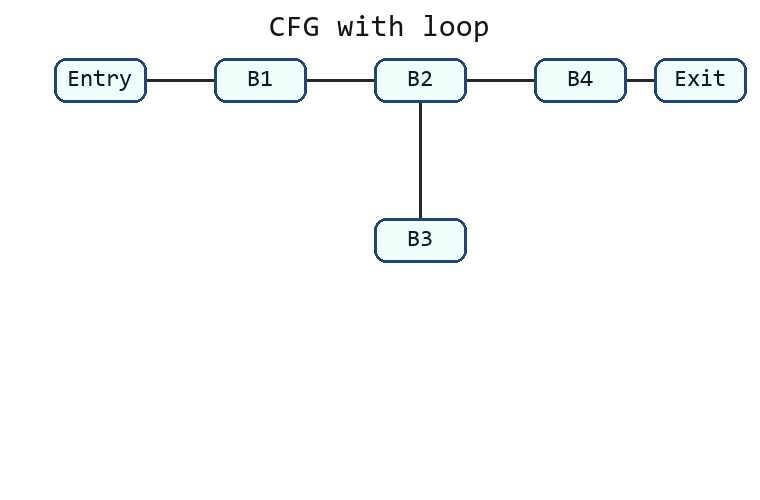
\includegraphics[width=0.82\linewidth]{figures/cfg-10-loop.png}
\par{\small CFG with loop}
\end{figure}

\paragraph*{1. Dom 集和 idom}

支配定义：若从 Entry 到结点 n 的每条路径都经过 d，则 d 支配 n。

Dom 集：

\begin{longtable}{|p{0.47\linewidth}|p{0.47\linewidth}|}
\hline
结点 & Dom \\
\hline
\endfirsthead
结点 & Dom \\
\hline
\endhead
Entry & \texttt{\textbackslash{}\{Entry\textbackslash{}\}} \\
\hline
B1 & \texttt{\textbackslash{}\{Entry,B1\textbackslash{}\}} \\
\hline
B2 & \texttt{\textbackslash{}\{Entry,B1,B2\textbackslash{}\}} \\
\hline
B3 & \texttt{\textbackslash{}\{Entry,B1,B2,B3\textbackslash{}\}} \\
\hline
B4 & \texttt{\textbackslash{}\{Entry,B1,B2,B4\textbackslash{}\}} \\
\hline
Exit & \texttt{\textbackslash{}\{Entry,B1,B2,B4,Exit\textbackslash{}\}} \\
\hline
\end{longtable}

直接支配者：

\begin{longtable}{|p{0.47\linewidth}|p{0.47\linewidth}|}
\hline
结点 & idom \\
\hline
\endfirsthead
结点 & idom \\
\hline
\endhead
B1 & Entry \\
\hline
B2 & B1 \\
\hline
B3 & B2 \\
\hline
B4 & B2 \\
\hline
Exit & B4 \\
\hline
\end{longtable}

\paragraph*{2. 支配树}

\begin{figure}[H]\centering
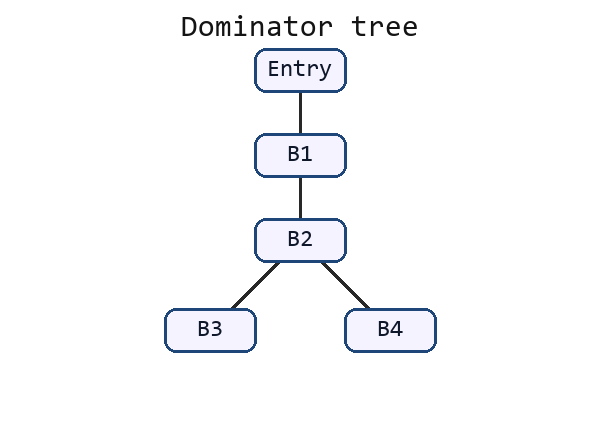
\includegraphics[width=0.82\linewidth]{figures/dom-tree-10.png}
\par{\small 支配树}
\end{figure}

\begin{Verbatim}[fontsize=\small,breaklines=true]
Entry
  B1
    B2
      B3
      B4
        Exit
\end{Verbatim}

\paragraph*{3. PostDom 集和 ipdom}

后支配定义：若从结点 n 到 Exit 的每条路径都经过 p，则 p 后支配 n。

\begin{longtable}{|p{0.47\linewidth}|p{0.47\linewidth}|}
\hline
结点 & PostDom \\
\hline
\endfirsthead
结点 & PostDom \\
\hline
\endhead
Exit & \texttt{\textbackslash{}\{Exit\textbackslash{}\}} \\
\hline
B4 & \texttt{\textbackslash{}\{B4,Exit\textbackslash{}\}} \\
\hline
B3 & \texttt{\textbackslash{}\{B3,B2,B4,Exit\textbackslash{}\}} \\
\hline
B2 & \texttt{\textbackslash{}\{B2,B4,Exit\textbackslash{}\}} \\
\hline
B1 & \texttt{\textbackslash{}\{B1,B2,B4,Exit\textbackslash{}\}} \\
\hline
Entry & \texttt{\textbackslash{}\{Entry,B1,B2,B4,Exit\textbackslash{}\}} \\
\hline
\end{longtable}

直接后支配者：

\begin{longtable}{|p{0.47\linewidth}|p{0.47\linewidth}|}
\hline
结点 & ipdom \\
\hline
\endfirsthead
结点 & ipdom \\
\hline
\endhead
Entry & B1 \\
\hline
B1 & B2 \\
\hline
B2 & B4 \\
\hline
B3 & B2 \\
\hline
B4 & Exit \\
\hline
\end{longtable}

\paragraph*{4. 回边和自然循环}

检查 CFG 中指向前面循环头的边：

\begin{Verbatim}[fontsize=\small,breaklines=true]
B3 -> B2
\end{Verbatim}

因为 \texttt{B2} 支配 \texttt{B3}，所以 \texttt{B3 -> B2} 是回边。

自然循环构造：

\begin{Verbatim}[fontsize=\small,breaklines=true]
从回边尾 B3 开始，反向沿前驱搜索，直到回边头 B2。
包含回边头 B2 和搜索到的所有结点。
\end{Verbatim}

结果：

\begin{Verbatim}[fontsize=\small,breaklines=true]
自然循环 = {B2, B3}
\end{Verbatim}

\paragraph*{5. 是否可归约}

该 CFG 可归约。依据：

\begin{Verbatim}[fontsize=\small,breaklines=true]
循环入口唯一，为 B2。
回边 B3 -> B2 的头 B2 支配尾 B3。
不存在多个入口进入同一个循环体的结构。
\end{Verbatim}
\end{document}
